% Standalone compile wrapper for ../background.tex (2026-05-30 STRUCTURAL rewrite).
% Compiles the structural-model walkthrough: six TikZ figures reused from
% figures_old.tex (paradigm-as-net, carry-over, derived conservatism, BMR
% precision-corner navigation, scalar-vs-structural headline, multi-agent),
% so the palette + tikz libraries below are figures_old.tex's, not the
% scalar pomdp_paradigm_model.tex's.
\documentclass[11pt,a4paper]{article}

\usepackage[utf8]{inputenc}
\usepackage[T1]{fontenc}
\usepackage[english]{babel}
\usepackage{amsmath,amssymb,mathtools,bm}
\usepackage{amsfonts}
\usepackage[round,authoryear]{natbib}
\usepackage{hyperref}
\usepackage[margin=1in]{geometry}
\usepackage{microtype}
\usepackage{xcolor}
\usepackage{tikz}
\usepackage{pgfplots}
\pgfplotsset{compat=1.18}
\usetikzlibrary{
  arrows.meta,
  positioning,
  decorations.pathmorphing,
  decorations.pathreplacing,
  decorations.markings,
  decorations.text,
  shapes.geometric,
  shapes.misc,
  fit,
  backgrounds,
  calc,
  patterns,
  intersections
}

\hypersetup{colorlinks=true, linkcolor=black, citecolor=blue, urlcolor=blue}

% --- Colour palette imported verbatim from figures_old.tex
\definecolor{coreblue}{RGB}{40, 70, 130}
\definecolor{coredeep}{RGB}{25, 50, 100}
\definecolor{paradigmA}{RGB}{170, 60, 60}
\definecolor{paradigmB}{RGB}{60, 130, 90}
\definecolor{softA}{RGB}{240, 215, 215}
\definecolor{softB}{RGB}{215, 235, 225}
\definecolor{softblue}{RGB}{215, 225, 240}
\definecolor{accentamber}{RGB}{200, 145, 50}
\definecolor{accentpurple}{RGB}{120, 80, 150}
\definecolor{softpurple}{RGB}{230, 220, 240}
\definecolor{softamber}{RGB}{245, 230, 200}
\definecolor{notegrey}{RGB}{95, 95, 110}
\definecolor{darkgrey}{RGB}{60, 60, 70}

% --- Math macros used by the walkthrough prose
\providecommand{\KL}[2]{D_{\mathrm{KL}}\!\left[#1\,\|\,#2\right]}
\providecommand{\E}[1]{\mathbb{E}\!\left[#1\right]}

\title{Background --- The Structural Paradigm Model\\[2pt]
       \large IWAI 2026: Paradigm Dynamics in Multi-Agent Motivated Belief}
\author{Hallgren \& Hyland}
\date{2026-05-30 (structural rewrite; scalar walkthrough archived as
      background\_scalar\_walkthrough.tex)}

\begin{document}
\maketitle

\noindent\textit{Step-by-step construction of the structural paradigm
model. A paradigm is a precision-weighted Bayes net of interdependent
commitments; conservatism is derived from structural position; paradigm
change is carry-over by message propagation; structural inference is
Bayesian model reduction over a continuous precision space; the
population signature is a graded structural reorganisation. The scalar
model is the baseline it departs from. Figures reused from
\texttt{figures\_old.tex}; the prior scalar and lit-review drafts are
preserved in this directory.}

\bigskip

% =====================================================================
% background.tex --- IWAI 2026, Hallgren & Hyland
% STRUCTURAL model walkthrough (2026-05-30 rewrite).
%
% Object: the paradigm is itself a precision-weighted Bayes net of
% interdependent commitments (core/belt). Conservatism is DERIVED from
% structural position; paradigm change is carry-over by message-passing;
% structural inference is Bayesian model reduction over a continuous
% precision space; the population signature is a continuous structural
% phase transition (graded belt-first/core-last reorganisation), NOT a
% damped oscillation to scalar consensus.
%
% Register: declarative strawman (no open-questions section). The scalar
% model is the baseline it departs from; it survives only as Fig 5's red
% curve.
%
% Figures: six TikZ blocks reused near-verbatim from figures_old.tex.
% Palette + tikz libraries live in the _build/main.tex wrapper.
%
% Predecessors archived in this directory: background_scalar_walkthrough.tex
% (the scalar walkthrough), background_litreview.tex (the survey).
%
% Citation keys: hand-curated keys resolve against paper/refs.bib;
% Author20XX_n keys are Semantic Scholar auto-keys from the cluster bibs.
% % TODO ADD marks foundational anchors still to be hand-added to refs.bib.
% =====================================================================

% =====================================================================
\section{The Phenomenon}
\label{sec:phenomenon}
% =====================================================================

Scientific communities revise their theoretical commitments more slowly
than the evidence alone would dictate, and when they move they move
abruptly and path-dependently \citep{kuhn1962Structure}. Kuhn's deepest
observation is that the paradigm shapes what a scientist can perceive,
what she chooses to investigate, and what alternatives she will
entertain --- three faces of one structural fact. The scalar reading of
this phenomenon --- a single categorical commitment $\theta$ revised
under a conservatism dial --- can reproduce the lag, but it represents
the paradigm as a point. A paradigm is not a point. It is a structured
web of interdependent commitments, and the cost of changing it is the
cost of re-reading every commitment that depends on the one that moved.
This document builds the model that takes that structure literally. Each
step introduces the formal object that answers the question its
predecessor leaves open.

% =====================================================================
\section*{Desiderata}
\addcontentsline{toc}{section}{Desiderata}
\label{sec:desiderata}
% =====================================================================

\noindent\fbox{\parbox{0.97\textwidth}{%
The construction must satisfy the following:
\begin{enumerate}\setlength{\itemsep}{2pt}\setlength{\topsep}{2pt}
\item \textbf{The paradigm is a structured object.} A paradigm is a
  Bayes net of interdependent commitments with a densely-connected core
  and a sparse belt in contact with observation --- not a categorical
  index.
\item \textbf{Carry-over.} Revising a commitment forces re-reading of
  everything that depends on it; the cost of paradigm change is the
  aggregate of these induced revisions, propagated through the network.
\item \textbf{Conservatism is derived, not assigned.} The resistance of
  each commitment to revision falls out of its structural position
  (core vs belt), rather than being parameterised by a global dial.
\item \textbf{Structural inference is principled.} Choosing among
  network structures is Bayesian model reduction over a continuous
  precision space whose corners are the discrete topologies.
\item \textbf{The population signature is a graded reorganisation.} The
  community does not flip a single variable at a threshold; it
  reorganises its joint network belt-first, core-last, producing a
  measurable graded order parameter --- the signature the scalar
  treatment cannot produce.
\item \textbf{Active-inference machinery, unmodified.} Variational and
  expected free energy \citep{friston2015ActiveInferenceEpistemic, millidge2021EFE} enter in standard form; structural utility extends
  \citet{hylandAlbarracin2025MindChange} from values to topology.
\end{enumerate}}}

% =====================================================================
\section{Building the Model}
\label{sec:walkthrough}
% =====================================================================

\subsection{Step 1: The paradigm is a structured object}
\label{ssec:structured}

\noindent\textit{What does the agent represent?} Not a categorical
$\theta$, but a paradigm network $G = (V, E, \Pi)$: nodes $v \in V$
carry theoretical commitments $x_v$; directed edges $(u\!\to\!v) \in E$
carry inferential dependencies; each edge has a coupling precision
$\pi_{uv} \in \Pi$ measuring how tightly the commitment at $v$ is bound
to the one at $u$. The internal coherence of the paradigm is a
precision-weighted graphical model,
\begin{equation}
p(x \mid G) \;\propto\;
\prod_{(u \to v) \in E} \psi_{uv}(x_u, x_v)^{\,\pi_{uv}},
\label{eq:net}
\end{equation}
so that strongly-coupled commitments (high $\pi$) must move together.
The \emph{core} is the densely-connected, high-precision interior; the
\emph{belt} $B \subset V$ is the sparse periphery in contact with
observation \citep{Heijdra1986_6, Ostapiuk2025_11, Wahyudi2026_2}. The
full generative model carries a fast world state $s_t$ with real
dynamics and the slow paradigm structure that conditions how the world
is read,
\begin{equation}
p(o_{1:T}, s_{1:T}, x, G)
= p(G)\,p(x \mid G)\!\prod_t p(o_t \mid s_t, x_B, G)\,
   p(s_t \mid s_{t-1}, a_{t-1}).
\label{eq:gen}
\end{equation}
Figure~\ref{fig:structured} contrasts the object the paper is about
with the scalar treatment it replaces.

\begin{figure}[t]
\centering
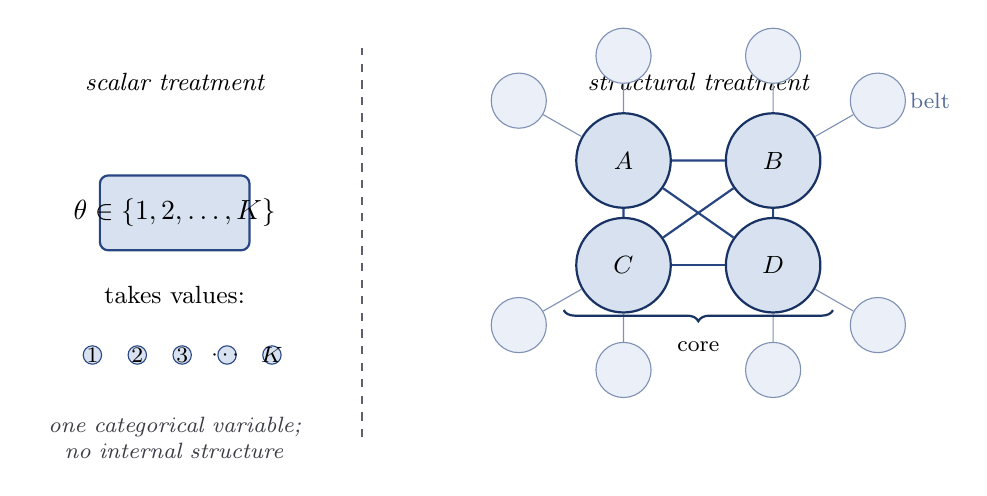
\begin{tikzpicture}[scale=0.95]
  % ---------- LEFT PANEL: scalar paradigm ----------
  \begin{scope}[xshift=0cm]
    \node[font=\small\itshape, anchor=north] at (1.5, 4.5) {scalar treatment};
    \draw[thick, coreblue, fill=softblue, rounded corners=3pt] (0.5, 2) rectangle (2.5, 3);
    \node at (1.5, 2.5) {$\theta \in \{1, 2, \ldots, K\}$};
    \node[font=\small] at (1.5, 1.4) {takes values:};
    \foreach \x/\v in {0.4/$1$, 1/$2$, 1.6/$3$, 2.2/$\cdots$, 2.8/$K$} {
      \draw[coreblue, fill=softblue] (\x, 0.6) circle (3.5pt);
      \node[font=\footnotesize] at (\x, 0.6) {\v};
    }
    \node[font=\footnotesize\itshape, anchor=north, text width=3.5cm, align=center, text=darkgrey]
      at (1.5, -0.1) {one categorical variable;\\ no internal structure};
  \end{scope}
  \draw[thick, dashed, notegrey] (4, -0.5) -- (4, 4.7);
  % ---------- RIGHT PANEL: structured paradigm ----------
  \begin{scope}[xshift=4.5cm]
    \node[font=\small\itshape, anchor=north] at (4, 4.5) {structural treatment};
    \node[circle, draw=coredeep, thick, fill=softblue, minimum size=12mm, font=\small] (A) at (3, 3.2) {$A$};
    \node[circle, draw=coredeep, thick, fill=softblue, minimum size=12mm, font=\small] (B) at (5, 3.2) {$B$};
    \node[circle, draw=coredeep, thick, fill=softblue, minimum size=12mm, font=\small] (C) at (3, 1.8) {$C$};
    \node[circle, draw=coredeep, thick, fill=softblue, minimum size=12mm, font=\small] (D) at (5, 1.8) {$D$};
    \draw[thick, coreblue] (A) -- (B);
    \draw[thick, coreblue] (A) -- (C);
    \draw[thick, coreblue] (A) -- (D);
    \draw[thick, coreblue] (B) -- (C);
    \draw[thick, coreblue] (B) -- (D);
    \draw[thick, coreblue] (C) -- (D);
    \node[circle, draw=coreblue!60, fill=softblue!50, minimum size=7mm, font=\footnotesize] (b1) at (1.6, 4.0) {};
    \node[circle, draw=coreblue!60, fill=softblue!50, minimum size=7mm, font=\footnotesize] (b2) at (6.4, 4.0) {};
    \node[circle, draw=coreblue!60, fill=softblue!50, minimum size=7mm, font=\footnotesize] (b3) at (1.6, 1.0) {};
    \node[circle, draw=coreblue!60, fill=softblue!50, minimum size=7mm, font=\footnotesize] (b4) at (6.4, 1.0) {};
    \node[circle, draw=coreblue!60, fill=softblue!50, minimum size=7mm, font=\footnotesize] (b5) at (3, 0.4) {};
    \node[circle, draw=coreblue!60, fill=softblue!50, minimum size=7mm, font=\footnotesize] (b6) at (5, 0.4) {};
    \node[circle, draw=coreblue!60, fill=softblue!50, minimum size=7mm, font=\footnotesize] (b7) at (3, 4.6) {};
    \node[circle, draw=coreblue!60, fill=softblue!50, minimum size=7mm, font=\footnotesize] (b8) at (5, 4.6) {};
    \draw[coreblue!60] (b1) -- (A);
    \draw[coreblue!60] (b2) -- (B);
    \draw[coreblue!60] (b3) -- (C);
    \draw[coreblue!60] (b4) -- (D);
    \draw[coreblue!60] (b5) -- (C);
    \draw[coreblue!60] (b6) -- (D);
    \draw[coreblue!60] (b7) -- (A);
    \draw[coreblue!60] (b8) -- (B);
    \draw[decorate, decoration={brace, amplitude=4pt, mirror}, thick, coredeep]
      (2.2, 1.2) -- (5.8, 1.2);
    \node[font=\footnotesize, anchor=north] at (4, 0.9) {core};
    \node[font=\footnotesize, anchor=west, text=coreblue!80] at (6.7, 4.0) {belt};
  \end{scope}
\end{tikzpicture}
\caption{The paradigm is not a scalar. Left: the scalar treatment ---
one categorical variable, no internal structure. Right: the structural
object the paper is about --- a Bayes net of commitments with a
densely-connected core and a sparse belt in contact with observation.
The right-hand panel carries inferential dependency the left cannot
represent.}
\label{fig:structured}
\end{figure}

\subsection{Step 2: Theory-laden perception through the belt}
\label{ssec:perception}

\noindent\textit{What makes the network a \emph{paradigm}?} The belt is
where the network meets the world: the observation likelihood in
Eq.~\eqref{eq:gen} is conditioned on the belt-node values $x_B$, which
are themselves downstream --- through the edges of
Eq.~\eqref{eq:net} --- of the core. Perception is therefore filtered
through the whole network. Two agents whose cores differ read the same
world state $s_t$ into different predicted observations, because the
core propagates to different belt activations and hence to different
likelihoods $p(o_t \mid s_t, x_B, G)$. This is theory-laden perception
made structural: the residue that resists deflation of incommensurability
is the difference between two generative \emph{networks}, not two values
of one variable \citep{Chang2012_9, Carrier2002_4, Malone1993_5}. What
counts as an anomaly versus a nuisance is the assignment the current
core forces on its belt.

\subsection{Step 3: Structural utility and the carry-over property}
\label{ssec:carryover}

\noindent\textit{Why is paradigm change expensive?} Not because a dial
is set high. \citet{hylandAlbarracin2025MindChange} give belief revision
a cost: a candidate update maximises a belief-utility net of a
complexity penalty, $q' = \arg\max_q \{ U[q] + \alpha\,\mathbb{E}_q[\log
L] - \lambda\,\mathrm{KL}[q \,\|\, q_0]\}$, with $\lambda$ a conservatism
on a scalar belief. In the structural model the object being revised is a
node value $x_v$ embedded in $G$, and a revision cannot stay local.
Setting $x_v \to x_v'$ emits precision-weighted messages along the edges
of Eq.~\eqref{eq:net}; each dependent node must re-equilibrate to restore
coherence; those re-equilibrations emit their own messages. The cost of
the revision is the aggregate of this propagation,
\begin{equation}
C(v) \;=\; \mathrm{KL}\!\left[q'(x_v) \,\|\, q(x_v)\right]
\;+\!\!\sum_{(v \to w) \in E}\!\! \pi_{vw}\,
   \mathbb{E}\!\left[\,\mathrm{KL}\!\left[q'(x_w) \,\|\, q(x_w)\right]\right]
\;+\;\cdots,
\label{eq:carryover}
\end{equation}
the local divergence plus the precision-weighted divergences of every
induced downstream revision, summed over the cascade. This is the
\emph{carry-over property}: the phlogistonian who becomes a Lavoisian
must revise combustion, calcination, mass conservation, and gas pressure
together, because they are literally connected. Carry-over is the
structural counterpart of Kuhnian incommensurability, made literal as
message propagation (Figure~\ref{fig:carryover}). The scalar conservatism
$\lambda$ is the degenerate single-node limit of
Eq.~\eqref{eq:carryover}, recovered when $E = \varnothing$. The
\emph{structural utility} extends \citet{hylandAlbarracin2025MindChange}
from values to topology,
\begin{equation}
U(G) \;=\; \sum_{(u \to v) \in E} u_{uv}\,\pi_{uv},
\label{eq:structutil}
\end{equation}
a preference over which edges are held at which precision --- a value
attached to keeping the core intact --- entering the revision score as a
term that resists precision changes lowering $U$.

\begin{figure}[t]
\centering
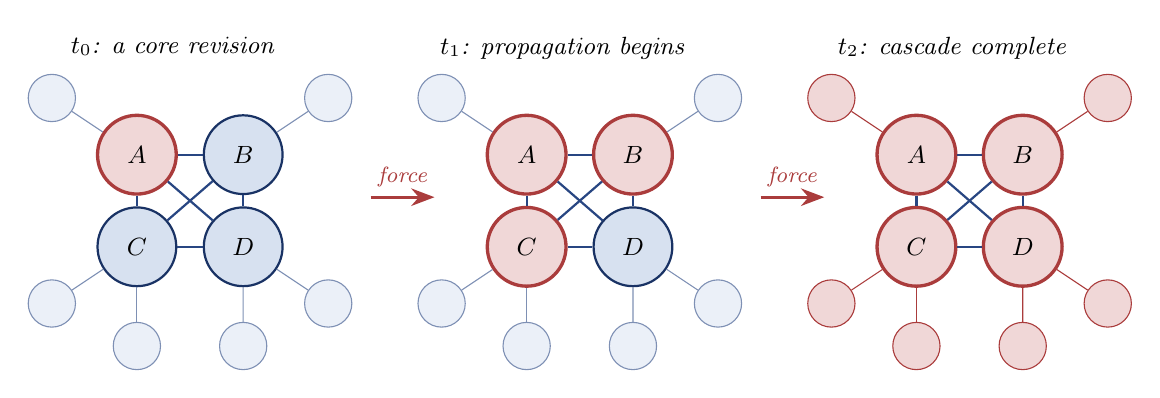
\begin{tikzpicture}[scale=0.9]
  \foreach \tx/\tlab/\activeA/\activeB/\activeC/\activeD/\activeBelt in {
    0/$t_0$: a core revision/1/0/0/0/0,
    5.5/$t_1$: propagation begins/1/1/1/0/0,
    11/$t_2$: cascade complete/1/1/1/1/1
  } {
    \begin{scope}[xshift=\tx cm]
      \node[font=\small\itshape, anchor=north] at (2, 5.2) {\tlab};
      \ifnum\activeA=1
        \node[circle, draw=paradigmA, very thick, fill=softA, minimum size=10mm, font=\small] (A) at (1.5, 3.4) {$A$};
      \else
        \node[circle, draw=coredeep, thick, fill=softblue, minimum size=10mm, font=\small] (A) at (1.5, 3.4) {$A$};
      \fi
      \ifnum\activeB=1
        \node[circle, draw=paradigmA, very thick, fill=softA, minimum size=10mm, font=\small] (B) at (3, 3.4) {$B$};
      \else
        \node[circle, draw=coredeep, thick, fill=softblue, minimum size=10mm, font=\small] (B) at (3, 3.4) {$B$};
      \fi
      \ifnum\activeC=1
        \node[circle, draw=paradigmA, very thick, fill=softA, minimum size=10mm, font=\small] (C) at (1.5, 2.1) {$C$};
      \else
        \node[circle, draw=coredeep, thick, fill=softblue, minimum size=10mm, font=\small] (C) at (1.5, 2.1) {$C$};
      \fi
      \ifnum\activeD=1
        \node[circle, draw=paradigmA, very thick, fill=softA, minimum size=10mm, font=\small] (D) at (3, 2.1) {$D$};
      \else
        \node[circle, draw=coredeep, thick, fill=softblue, minimum size=10mm, font=\small] (D) at (3, 2.1) {$D$};
      \fi
      \draw[thick, coreblue] (A) -- (B);
      \draw[thick, coreblue] (A) -- (C);
      \draw[thick, coreblue] (A) -- (D);
      \draw[thick, coreblue] (B) -- (C);
      \draw[thick, coreblue] (B) -- (D);
      \draw[thick, coreblue] (C) -- (D);
      \ifnum\activeBelt=1
        \def\beltcolour{paradigmA}
        \def\beltfill{softA}
      \else
        \def\beltcolour{coreblue!60}
        \def\beltfill{softblue!50}
      \fi
      \node[circle, draw=\beltcolour, fill=\beltfill, minimum size=6mm, font=\footnotesize] (b1) at (0.3, 4.2) {};
      \node[circle, draw=\beltcolour, fill=\beltfill, minimum size=6mm, font=\footnotesize] (b2) at (4.2, 4.2) {};
      \node[circle, draw=\beltcolour, fill=\beltfill, minimum size=6mm, font=\footnotesize] (b3) at (0.3, 1.3) {};
      \node[circle, draw=\beltcolour, fill=\beltfill, minimum size=6mm, font=\footnotesize] (b4) at (4.2, 1.3) {};
      \node[circle, draw=\beltcolour, fill=\beltfill, minimum size=6mm, font=\footnotesize] (b5) at (1.5, 0.7) {};
      \node[circle, draw=\beltcolour, fill=\beltfill, minimum size=6mm, font=\footnotesize] (b6) at (3, 0.7) {};
      \draw[\beltcolour] (b1) -- (A);
      \draw[\beltcolour] (b2) -- (B);
      \draw[\beltcolour] (b3) -- (C);
      \draw[\beltcolour] (b4) -- (D);
      \draw[\beltcolour] (b5) -- (C);
      \draw[\beltcolour] (b6) -- (D);
    \end{scope}
  }
  \draw[->, very thick, paradigmA, >=Stealth] (4.8, 2.8) -- (5.7, 2.8)
    node[midway, above, font=\footnotesize\itshape] {force};
  \draw[->, very thick, paradigmA, >=Stealth] (10.3, 2.8) -- (11.2, 2.8)
    node[midway, above, font=\footnotesize\itshape] {force};
\end{tikzpicture}
\caption{The carry-over property. A value change at the core (red)
propagates outward along the inferential edges, forcing re-reading of
every dependent commitment. The propagation is not a choice but a
consequence of the structural commitments (arrows: ``force''); its
integrated cost is Eq.~\eqref{eq:carryover}. This is the move the scalar
treatment cannot represent.}
\label{fig:carryover}
\end{figure}

\subsection{Step 4: Conservatism falls out of structure}
\label{ssec:conservatism}

\noindent\textit{Where does the conservatism gradient come from?} From
the graph, not from assignment. Reading Eq.~\eqref{eq:carryover} as a
per-node quantity, the conservatism of node $i$ is the precision-weighted
cost of moving it through the message-passing,
\begin{equation}
\lambda_i \;=\;\!\! \sum_{w \in \mathrm{desc}(i)}\!\! \pi_{i \rightsquigarrow w},
\label{eq:lambda}
\end{equation}
the sum over $i$'s descendants of the precision along the path
connecting them. A core node has many high-precision descendants and is
therefore expensive to revise; a belt node has few and is cheap. No
$\lambda$ is assigned: the gradient of Figure~\ref{fig:conservatism} is
the connectivity of the network, read off directly. The intermediate
shell $M_i$ makes the gradient continuous rather than binary --- which
is what the continuous structural inference of the next step requires.

\begin{figure}[t]
\centering
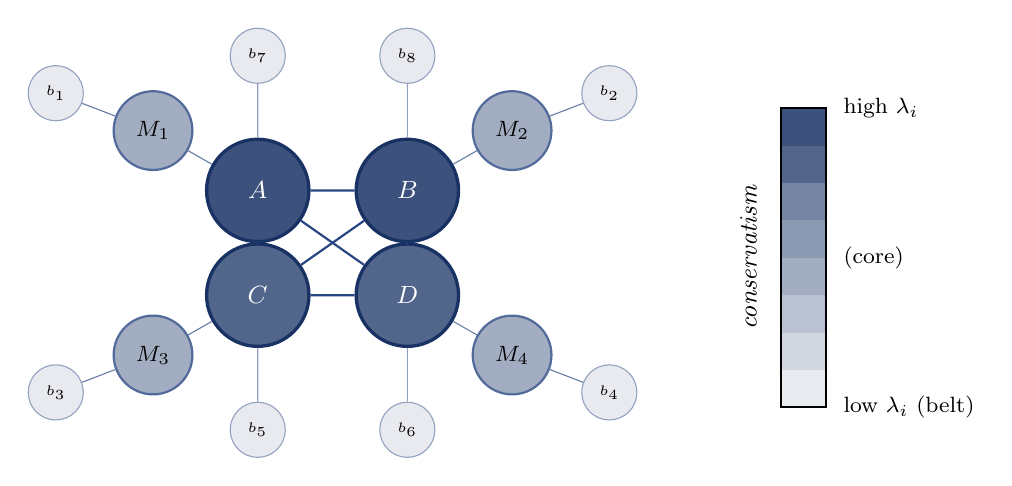
\begin{tikzpicture}[scale=0.95]
  \node[circle, draw=coredeep, very thick, fill=coredeep!85, minimum size=13mm, font=\small, text=white] (A) at (3, 3.4) {$A$};
  \node[circle, draw=coredeep, very thick, fill=coredeep!85, minimum size=13mm, font=\small, text=white] (B) at (5, 3.4) {$B$};
  \node[circle, draw=coredeep, very thick, fill=coredeep!75, minimum size=13mm, font=\small, text=white] (C) at (3, 2.0) {$C$};
  \node[circle, draw=coredeep, very thick, fill=coredeep!75, minimum size=13mm, font=\small, text=white] (D) at (5, 2.0) {$D$};
  \draw[thick, coreblue] (A) -- (B);
  \draw[thick, coreblue] (A) -- (C);
  \draw[thick, coreblue] (A) -- (D);
  \draw[thick, coreblue] (B) -- (C);
  \draw[thick, coreblue] (B) -- (D);
  \draw[thick, coreblue] (C) -- (D);
  \node[circle, draw=coreblue!80, thick, fill=coredeep!40, minimum size=10mm, font=\footnotesize] (m1) at (1.6, 4.2) {$M_1$};
  \node[circle, draw=coreblue!80, thick, fill=coredeep!40, minimum size=10mm, font=\footnotesize] (m2) at (6.4, 4.2) {$M_2$};
  \node[circle, draw=coreblue!80, thick, fill=coredeep!40, minimum size=10mm, font=\footnotesize] (m3) at (1.6, 1.2) {$M_3$};
  \node[circle, draw=coreblue!80, thick, fill=coredeep!40, minimum size=10mm, font=\footnotesize] (m4) at (6.4, 1.2) {$M_4$};
  \node[circle, draw=coreblue!50, fill=coredeep!10, minimum size=7mm, font=\tiny] (b1) at (0.3, 4.7) {$b_1$};
  \node[circle, draw=coreblue!50, fill=coredeep!10, minimum size=7mm, font=\tiny] (b2) at (7.7, 4.7) {$b_2$};
  \node[circle, draw=coreblue!50, fill=coredeep!10, minimum size=7mm, font=\tiny] (b3) at (0.3, 0.7) {$b_3$};
  \node[circle, draw=coreblue!50, fill=coredeep!10, minimum size=7mm, font=\tiny] (b4) at (7.7, 0.7) {$b_4$};
  \node[circle, draw=coreblue!50, fill=coredeep!10, minimum size=7mm, font=\tiny] (b5) at (3, 0.2) {$b_5$};
  \node[circle, draw=coreblue!50, fill=coredeep!10, minimum size=7mm, font=\tiny] (b6) at (5, 0.2) {$b_6$};
  \node[circle, draw=coreblue!50, fill=coredeep!10, minimum size=7mm, font=\tiny] (b7) at (3, 5.2) {$b_7$};
  \node[circle, draw=coreblue!50, fill=coredeep!10, minimum size=7mm, font=\tiny] (b8) at (5, 5.2) {$b_8$};
  \draw[coreblue!70] (b1) -- (m1);
  \draw[coreblue!70] (b2) -- (m2);
  \draw[coreblue!70] (b3) -- (m3);
  \draw[coreblue!70] (b4) -- (m4);
  \draw[coreblue!50] (b5) -- (C);
  \draw[coreblue!50] (b6) -- (D);
  \draw[coreblue!50] (b7) -- (A);
  \draw[coreblue!50] (b8) -- (B);
  \draw[coreblue!70] (m1) -- (A);
  \draw[coreblue!70] (m2) -- (B);
  \draw[coreblue!70] (m3) -- (C);
  \draw[coreblue!70] (m4) -- (D);
  \begin{scope}[xshift=10cm, yshift=0.5cm]
    \foreach \y/\op in {0/10, 0.5/20, 1/30, 1.5/40, 2/50, 2.5/60, 3/75, 3.5/85} {
      \fill[coredeep, opacity=0.01*\op] (0, \y) rectangle (0.6, \y+0.5);
    }
    \draw[thick] (0, 0) rectangle (0.6, 4);
    \node[font=\footnotesize, anchor=west] at (0.7, 4) {high $\lambda_i$};
    \node[font=\footnotesize, anchor=west] at (0.7, 2) {(core)};
    \node[font=\footnotesize, anchor=west] at (0.7, 0) {low $\lambda_i$ (belt)};
    \node[font=\small\itshape, anchor=south, rotate=90] at (-0.2, 2) {conservatism};
  \end{scope}
\end{tikzpicture}
\caption{Conservatism is derived, not assigned. Colour saturation
encodes $\lambda_i$ (Eq.~\ref{eq:lambda}): high in the core, which has
many high-precision descendants; low in the belt, which has few. The
intermediate shell $M_i$ makes the gradient continuous.}
\label{fig:conservatism}
\end{figure}

\subsection{Step 5: BMR as precision-corner navigation}
\label{ssec:bmr}

\noindent\textit{How does the agent choose among network structures?}
Structural inference --- scoring alternative graphs, not just alternative
values --- is Bayesian model reduction \citep{Friston2018_2, fristonPenny2011PostHocBMS}.% TODO ADD fristonPenny2011PostHocBMS
Once the full model is inverted, the evidence of any reduced model
differing only in its priors is available in closed form from the full
posterior and the prior ratio, generalising the Savage--Dickey density
ratio. Pruning edge $e$ corresponds to tightening the prior precision
$\lambda_e$ on its parameter toward infinity (the parameter is pinned,
the edge vanishes); freeing it corresponds to $\lambda_e \to 0$. The
change in variational free energy,
\begin{equation}
\Delta F_e \;=\; \ln \frac{\tilde p(o)}{p(o)}
\;-\; \Delta U(G),
\label{eq:bmr}
\end{equation}
is the log Bayes factor for the structural revision, net of the
structural-utility change from Eq.~\eqref{eq:structutil}; the agent
accepts the revision when $\Delta F_e > 0$. The discrete topologies are
the corners of a continuous precision space, and the interior is the
relaxation: partial edges, soft structural commitments. A structural
revision is a \emph{trajectory through the interior}
(Figure~\ref{fig:bmr}), never a discrete jump --- and that continuity is
exactly what produces the graded population dynamics of
Section~\ref{sec:result}.\footnote{The BMR prior precision $\lambda_e$
on an edge parameter (high $\Rightarrow$ edge pruned) runs opposite to
the coupling precision $\pi_{uv}$ of Eq.~\eqref{eq:net} (high
$\Rightarrow$ edge strong); a strongly coupled edge is one BMR keeps. It
is distinct again from the node conservatism $\lambda_i$ of
Eq.~\eqref{eq:lambda}.}

\begin{figure}[t]
\centering
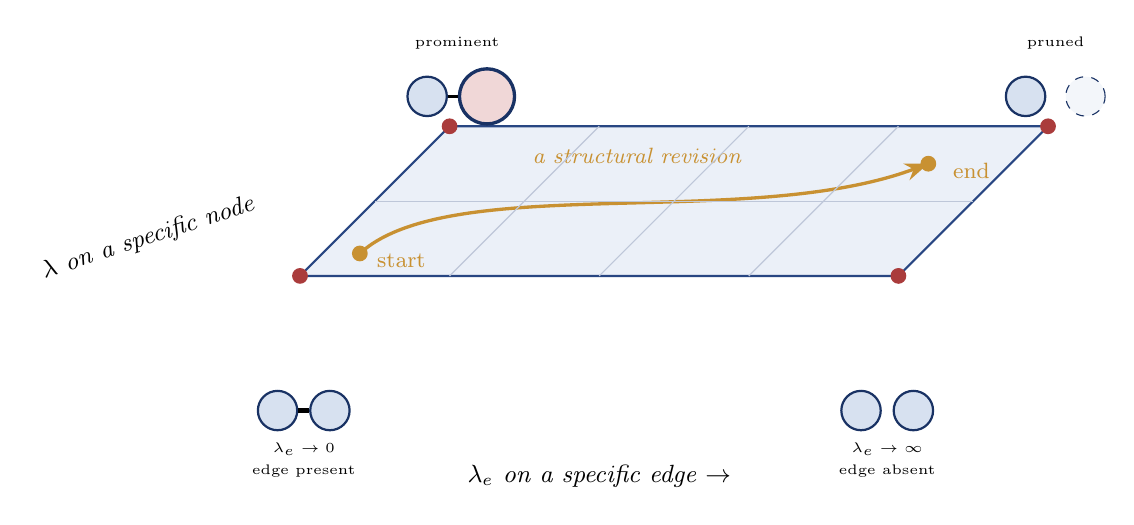
\begin{tikzpicture}[scale=0.95]
  \draw[thick, coreblue, fill=softblue!50] (0, 0) -- (8, 0) -- (10, 2) -- (2, 2) -- cycle;
  \begin{scope}[xshift=-0.3cm, yshift=-1.8cm]
    \node[circle, draw=coredeep, thick, fill=softblue, minimum size=5mm, font=\tiny] (a1) at (0, 0) {};
    \node[circle, draw=coredeep, thick, fill=softblue, minimum size=5mm, font=\tiny] (a2) at (0.7, 0) {};
    \draw[line width=1.5pt] (a1) -- (a2);
    \node[font=\tiny, anchor=north] at (0.35, -0.3) {$\lambda_e \to 0$};
    \node[font=\tiny, anchor=north] at (0.35, -0.6) {edge present};
  \end{scope}
  \begin{scope}[xshift=7.5cm, yshift=-1.8cm]
    \node[circle, draw=coredeep, thick, fill=softblue, minimum size=5mm, font=\tiny] (a3) at (0, 0) {};
    \node[circle, draw=coredeep, thick, fill=softblue, minimum size=5mm, font=\tiny] (a4) at (0.7, 0) {};
    \node[font=\tiny, anchor=north] at (0.35, -0.3) {$\lambda_e \to \infty$};
    \node[font=\tiny, anchor=north] at (0.35, -0.6) {edge absent};
  \end{scope}
  \begin{scope}[xshift=1.7cm, yshift=2.4cm]
    \node[circle, draw=coredeep, thick, fill=softblue, minimum size=5mm, font=\tiny] (a5) at (0, 0) {};
    \node[circle, draw=coredeep, very thick, fill=softA, minimum size=7mm, font=\tiny] (a6) at (0.8, 0) {};
    \draw[line width=1.2pt] (a5) -- (a6);
    \node[font=\tiny, anchor=south] at (0.4, 0.5) {prominent};
  \end{scope}
  \begin{scope}[xshift=9.7cm, yshift=2.4cm]
    \node[circle, draw=coredeep, thick, fill=softblue, minimum size=5mm, font=\tiny] (a7) at (0, 0) {};
    \node[circle, draw=coredeep, dashed, fill=softblue!30, minimum size=5mm, font=\tiny] (a8) at (0.8, 0) {};
    \node[font=\tiny, anchor=south] at (0.4, 0.5) {pruned};
  \end{scope}
  \fill[paradigmA] (0, 0) circle (3pt);
  \fill[paradigmA] (8, 0) circle (3pt);
  \fill[paradigmA] (2, 2) circle (3pt);
  \fill[paradigmA] (10, 2) circle (3pt);
  \node[font=\small\itshape, anchor=north] at (4, -2.4) {$\lambda_e$ on a specific edge $\to$};
  \node[font=\small\itshape, anchor=east, rotate=18] at (-0.5, 1) {$\lambda$ on a specific node};
  \draw[->, very thick, accentamber, >=Stealth]
    (0.8, 0.3) .. controls (2, 1.4) and (6, 0.6) .. (8.4, 1.5);
  \fill[accentamber] (0.8, 0.3) circle (3pt);
  \node[font=\footnotesize, accentamber, anchor=west] at (0.9, 0.2) {start};
  \fill[accentamber] (8.4, 1.5) circle (3pt);
  \node[font=\footnotesize, accentamber, anchor=west] at (8.6, 1.4) {end};
  \node[font=\footnotesize\itshape, accentamber] at (4.5, 1.6) {a structural revision};
  \foreach \x in {2, 4, 6} {
    \draw[coreblue!30, thin] (\x, 0) -- (\x+2, 2);
  }
  \draw[coreblue!30, thin] (1, 1) -- (9, 1);
\end{tikzpicture}
\vspace{1.4cm}
\caption{BMR as navigation through a continuous precision space. The
corners are discrete Bayes-net topologies (edges present at
$\lambda_e\!\to\!0$, absent at $\lambda_e\!\to\!\infty$); the interior is
partial edges and soft structural commitments. A structural revision
(amber) is a trajectory through the interior, scored by
Eq.~\eqref{eq:bmr} --- never a discrete jump. The continuity is what
enables the graded transition of Figure~\ref{fig:transition}.}
\label{fig:bmr}
\end{figure}

\noindent Appendix~\ref{app:abc} walks this reduction through concretely
for three competing paradigms $A$, $B$, $C$, with the carry-over of
Step~3 supplying the cost of the structural edit.

\subsection{Step 6: Active sampling under expected free energy}
\label{ssec:efe}

\noindent\textit{Which experiments does the agent run?} Observation is
an active decision: the agent allocates a finite precision budget across
belt nodes, selecting actions by expected free energy
\citep{friston2015ActiveInferenceEpistemic, millidge2021EFE, Mirza2019_2},
$G(a) = -\,\mathbb{E}[\log p(o \mid C)] + \mathbb{E}[\mathrm{KL}[q(\cdot
\mid o, a)\,\|\,q(\cdot)]]$, where the epistemic term now scores how much
an observation could license a \emph{structural} revision --- a change
of edge or node the agent actually entertains. The structural utility of
Eq.~\eqref{eq:structutil} tilts the planning belief, so experiments that
would force expensive core revisions appear risky and are under-sampled
\citep{feldmanFriston2010Attention, parrFriston2017Attention, parrFriston2019AdvancedAtt, limanowskiFriston2018Dark}. The three
Kuhnian faces are now one construction: perception is the belt
likelihood (Step~2); experimentation is this EFE policy; the reachable
hypothesis space is bounded by the carry-over cost (Steps~3--4), which
makes deep revisions nominally available but practically unreachable. No
face is an added bias term.

\subsection{Step 7: Multi-agent coupling of structured beliefs}
\label{ssec:multiagent}

\noindent\textit{What does a peer transmit?} Not a scalar opinion: a
candidate \emph{structural revision}. Each agent carries its own network
$G_a$; communication emits candidate edge- and node-revisions, and the
receiver imports them weighted by the trust-channel precision $\pi_s$ on
that link (Figure~\ref{fig:multiagent}). The scalar trust matrix $T$
mixing scalar beliefs is replaced by precision-weighted structural
exchange. The distinction the scalar model could only assert now falls
out of the representation: a \emph{bubble} is a missing channel
(topological absence --- exposure dissolves it); a \emph{chamber} is a
channel present but with $\pi_s \approx 0$ (precision suppression ---
exposure reinforces it) \citep{Nguyen2018_1, Pollock2024_3, Turner2023_2}.
Structural utility reappears at population scale: agents valuing their
current core assign low $\pi_s$ to channels carrying revisions to it ---
the network-level analogue of individual motivated attention
\citep{albarracin2022EpistemicCommunities}.

\begin{figure}[t]
\centering
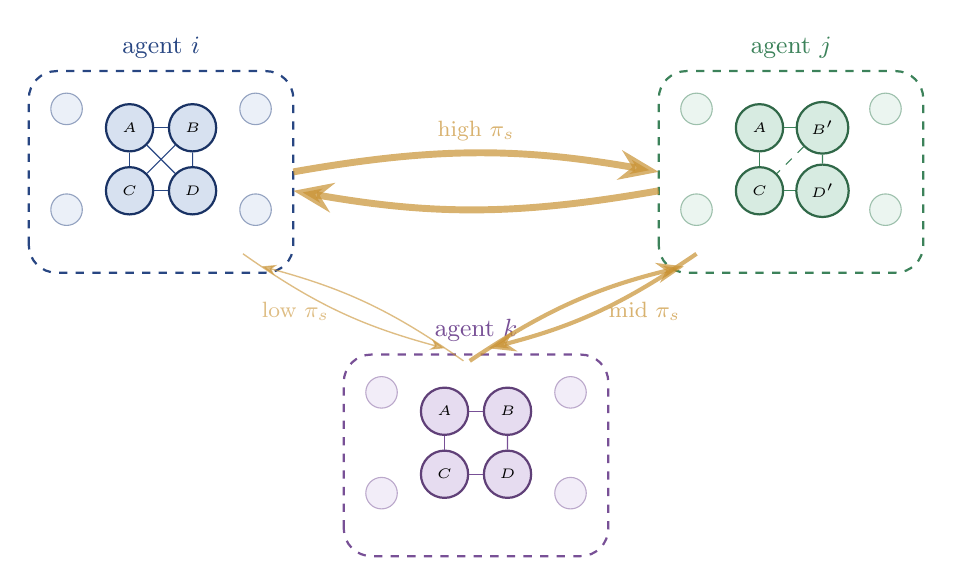
\begin{tikzpicture}[scale=0.8]
  % AGENT i - top left
  \begin{scope}[xshift=0cm, yshift=4cm]
    \draw[thick, coreblue, dashed, rounded corners=10pt] (-1.6, -1.6) rectangle (2.6, 1.6);
    \node[font=\small, coreblue, anchor=south] at (0.5, 1.65) {agent $i$};
    \node[circle, draw=coredeep, thick, fill=softblue, minimum size=6mm, font=\tiny] (i1) at (0, 0.7) {$A$};
    \node[circle, draw=coredeep, thick, fill=softblue, minimum size=6mm, font=\tiny] (i2) at (1, 0.7) {$B$};
    \node[circle, draw=coredeep, thick, fill=softblue, minimum size=6mm, font=\tiny] (i3) at (0, -0.3) {$C$};
    \node[circle, draw=coredeep, thick, fill=softblue, minimum size=6mm, font=\tiny] (i4) at (1, -0.3) {$D$};
    \draw[coreblue] (i1) -- (i2);
    \draw[coreblue] (i1) -- (i3);
    \draw[coreblue] (i2) -- (i4);
    \draw[coreblue] (i3) -- (i4);
    \draw[coreblue] (i1) -- (i4);
    \draw[coreblue] (i2) -- (i3);
    \node[circle, draw=coreblue!50, fill=softblue!50, minimum size=4mm] at (-1, 1) {};
    \node[circle, draw=coreblue!50, fill=softblue!50, minimum size=4mm] at (2, 1) {};
    \node[circle, draw=coreblue!50, fill=softblue!50, minimum size=4mm] at (-1, -0.6) {};
    \node[circle, draw=coreblue!50, fill=softblue!50, minimum size=4mm] at (2, -0.6) {};
  \end{scope}
  % AGENT j - top right
  \begin{scope}[xshift=10cm, yshift=4cm]
    \draw[thick, paradigmB, dashed, rounded corners=10pt] (-1.6, -1.6) rectangle (2.6, 1.6);
    \node[font=\small, paradigmB, anchor=south] at (0.5, 1.65) {agent $j$};
    \node[circle, draw=paradigmB!80!black, thick, fill=softB, minimum size=6mm, font=\tiny] (j1) at (0, 0.7) {$A$};
    \node[circle, draw=paradigmB!80!black, thick, fill=softB, minimum size=6mm, font=\tiny] (j2) at (1, 0.7) {$B'$};
    \node[circle, draw=paradigmB!80!black, thick, fill=softB, minimum size=6mm, font=\tiny] (j3) at (0, -0.3) {$C$};
    \node[circle, draw=paradigmB!80!black, thick, fill=softB, minimum size=6mm, font=\tiny] (j4) at (1, -0.3) {$D'$};
    \draw[paradigmB] (j1) -- (j2);
    \draw[paradigmB] (j1) -- (j3);
    \draw[paradigmB] (j2) -- (j4);
    \draw[paradigmB] (j3) -- (j4);
    \draw[paradigmB, dashed] (j2) -- (j3);
    \node[circle, draw=paradigmB!50, fill=softB!50, minimum size=4mm] at (-1, 1) {};
    \node[circle, draw=paradigmB!50, fill=softB!50, minimum size=4mm] at (2, 1) {};
    \node[circle, draw=paradigmB!50, fill=softB!50, minimum size=4mm] at (-1, -0.6) {};
    \node[circle, draw=paradigmB!50, fill=softB!50, minimum size=4mm] at (2, -0.6) {};
  \end{scope}
  % AGENT k - bottom centre
  \begin{scope}[xshift=5cm, yshift=-0.5cm]
    \draw[thick, accentpurple, dashed, rounded corners=10pt] (-1.6, -1.6) rectangle (2.6, 1.6);
    \node[font=\small, accentpurple, anchor=south] at (0.5, 1.65) {agent $k$};
    \node[circle, draw=accentpurple!80!black, thick, fill=softpurple, minimum size=6mm, font=\tiny] (k1) at (0, 0.7) {$A$};
    \node[circle, draw=accentpurple!80!black, thick, fill=softpurple, minimum size=6mm, font=\tiny] (k2) at (1, 0.7) {$B$};
    \node[circle, draw=accentpurple!80!black, thick, fill=softpurple, minimum size=6mm, font=\tiny] (k3) at (0, -0.3) {$C$};
    \node[circle, draw=accentpurple!80!black, thick, fill=softpurple, minimum size=6mm, font=\tiny] (k4) at (1, -0.3) {$D$};
    \draw[accentpurple] (k1) -- (k2);
    \draw[accentpurple] (k1) -- (k3);
    \draw[accentpurple] (k2) -- (k4);
    \draw[accentpurple] (k3) -- (k4);
    \node[circle, draw=accentpurple!50, fill=softpurple!50, minimum size=4mm] at (-1, 1) {};
    \node[circle, draw=accentpurple!50, fill=softpurple!50, minimum size=4mm] at (2, 1) {};
    \node[circle, draw=accentpurple!50, fill=softpurple!50, minimum size=4mm] at (-1, -0.6) {};
    \node[circle, draw=accentpurple!50, fill=softpurple!50, minimum size=4mm] at (2, -0.6) {};
  \end{scope}
  \draw[->, line width=2.5pt, accentamber, >=Stealth, opacity=0.7]
    (2.6, 4) to[bend left=10] node[midway, above, font=\footnotesize, sloped] {high $\pi_s$} (8.4, 4);
  \draw[<-, line width=2.5pt, accentamber, >=Stealth, opacity=0.7]
    (2.6, 3.7) to[bend right=10] (8.4, 3.7);
  \draw[->, line width=0.5pt, accentamber, >=Stealth, opacity=0.6]
    (1.8, 2.7) to[bend right=10] node[midway, left, font=\footnotesize] {low $\pi_s$} (5, 1.2);
  \draw[<-, line width=0.5pt, accentamber, >=Stealth, opacity=0.6]
    (2.1, 2.5) to[bend left=10] (5.3, 1.0);
  \draw[->, line width=1.5pt, accentamber, >=Stealth, opacity=0.7]
    (9, 2.7) to[bend left=10] node[midway, right, font=\footnotesize] {mid $\pi_s$} (5.7, 1.2);
  \draw[<-, line width=1.5pt, accentamber, >=Stealth, opacity=0.7]
    (8.8, 2.5) to[bend right=10] (5.4, 1.0);
\end{tikzpicture}
\caption{Multi-agent coupling with structured beliefs. Each agent
carries a full paradigm network; $i$ and $k$ share a structure, $j$
differs (primed nodes $B'$, $D'$ and a different $B'$--$C$ edge). Trust
precision $\pi_s$ on each channel (line thickness) sets how much weight a
receiver gives to candidate structural revisions from a neighbour. A
missing channel is a bubble; a present channel with $\pi_s\!\approx\!0$
is a chamber.}
\label{fig:multiagent}
\end{figure}

% =====================================================================
\section{The Central Result: Scalar Cascade versus Structural Reorganisation}
\label{sec:result}
% =====================================================================

\noindent\textit{What does the population do?} Define the order parameter
\begin{equation}
m(t) \;=\; \frac{1}{N}\sum_{a=1}^{N}
   \frac{\sum_{e \in E_a} \pi_e\,\mathbb{1}[\,e \text{ re-equilibrated to rival}\,]}
        {\sum_{e \in E_a} \pi_e},
\label{eq:order}
\end{equation}
the population-mean precision-weighted fraction of each agent's network
that has reorganised to the rival paradigm. The scalar model predicts a
single sharp cascade: there is one variable to flip, so $m(t)$ has one
inflection at threshold. The structural model predicts a graded
reorganisation: cheap belt revisions (low $\lambda_i$,
Eq.~\ref{eq:lambda}) happen first, the densely-connected core (high
$\lambda_i$) moves last, and $m(t)$ approaches its limit through a
sequence of smaller transitions whose internal structure is empirically
measurable (Figure~\ref{fig:transition}). The continuity of the precision
space (Step~5) is what makes the structural curve a graded approach
rather than a jump. This is the signature the scalar treatment cannot
produce.

\begin{figure}[t]
\centering
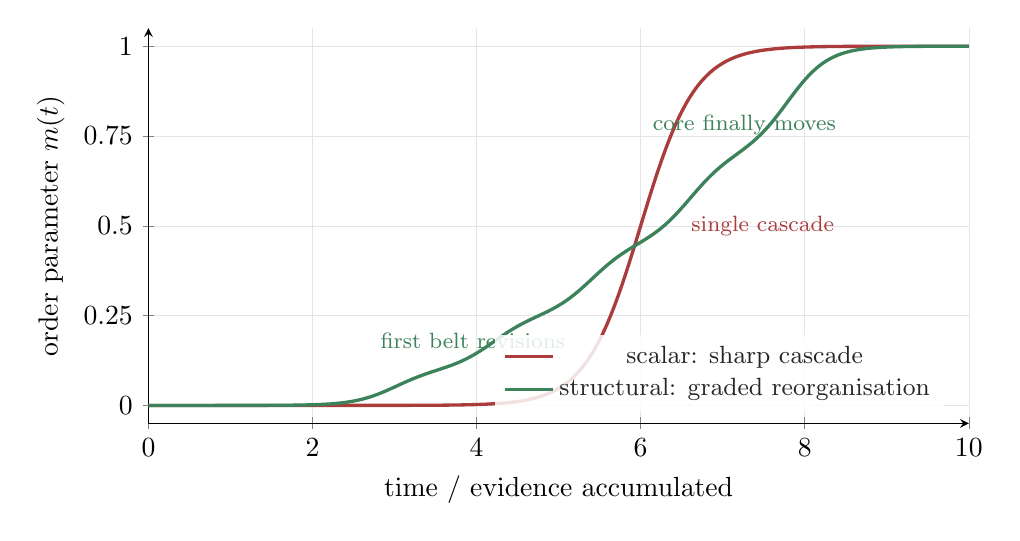
\begin{tikzpicture}
\begin{axis}[
  width=12cm, height=6.6cm,
  xlabel={time / evidence accumulated},
  ylabel={order parameter $m(t)$},
  xmin=0, xmax=10, ymin=-0.05, ymax=1.05,
  xtick={0, 2, 4, 6, 8, 10},
  ytick={0, 0.25, 0.5, 0.75, 1},
  grid=major,
  grid style={gray!20, very thin},
  legend pos=south east,
  legend style={font=\small, draw=none, fill=white, fill opacity=0.85},
  axis lines=left,
  every axis plot/.append style={very thick},
]
  \addplot[paradigmA, smooth, samples=200, domain=0:10]
    {1/(1+exp(-3*(x-6)))};
  \addlegendentry{scalar: sharp cascade}
  \addplot[paradigmB, smooth, samples=400, domain=0:10]
    {0.1/(1+exp(-4*(x-3.0))) +
     0.15/(1+exp(-4*(x-4.2))) +
     0.2/(1+exp(-4*(x-5.4))) +
     0.25/(1+exp(-4*(x-6.6))) +
     0.3/(1+exp(-4*(x-7.8)))};
  \addlegendentry{structural: graded reorganisation}
  \node[font=\footnotesize, paradigmA, anchor=west] at (axis cs:6.5, 0.5) {single cascade};
  \node[font=\footnotesize, paradigmB, anchor=east] at (axis cs:5.2, 0.18) {first belt revisions};
  \node[font=\footnotesize, paradigmB, anchor=east] at (axis cs:8.5, 0.78) {core finally moves};
\end{axis}
\end{tikzpicture}
\caption{The central empirical contrast (schematic; to be replaced with
simulation output). Both curves reach unity; the difference is the shape
of the approach. The scalar order parameter has one inflection ---
nothing to reorganise, one variable to flip. The structural order
parameter (Eq.~\ref{eq:order}) is a graded staircase: belt revisions are
cheap and early, the core is expensive and late. The internal structure
of the green curve is the measurable signature the structural extension
exists to produce.}
\label{fig:transition}
\end{figure}

The results the network-epistemology literature has accumulated as
separate findings recover from this one mechanism. The Zollman
speed--accuracy tradeoff% TODO ADD zollman2007NetworkEpistemology
is the topological statement of how the algebraic connectivity of the
trust graph governs the transient: denser graphs run the reorganisation
faster but lose the transient structural diversity that protects against
locking onto the worse paradigm. Paradoxical stubbornness --- the
regularising effect of high-$\lambda_i$ agents --- is the same fact read
at the agent level. The bubble-versus-chamber distinction
\citep{Nguyen2018_1} is the formal separation between sparsity of the
trust channels and the precision $\pi_s$ they carry. The structural model
does not stipulate these phenomena; it produces them.

% =====================================================================
\section{Discussion}
\label{sec:discussion}
% =====================================================================

The structural object buys what the scalar dial cannot: a paradigm whose
internal dependencies are explicit, a conservatism gradient that is
derived rather than assigned, a cost of paradigm change that is the
literal re-reading of dependent commitments, and a population signature
--- the graded reorganisation of Figure~\ref{fig:transition} --- that is
distinct from a damped oscillation to consensus and is the measurable
prediction the model exists to make. The scalar treatment is the
baseline: it is the degenerate single-node limit recovered when the
paradigm has no internal structure.

One extension is immediate. Throughout, the agent's policy over which
structural revisions it ever encounters is endogenous. In contemporary
practice it is not: citation recommenders, ranking, and institutional
visibility filters increasingly mediate which candidate revisions reach
a scientist at all \citep{kulveit2025GradualDisempowerment, critchKrueger2020ARCHES}. A curator intervening on the trust channels
supplies a third lever on $\pi_s$ beyond the agent and its neighbours,
and the structural model is the natural setting in which to ask whether
that curation merely renormalises the existing dynamics or installs new
attractors that survive cross-surprisal because the disconfirming
revisions are never sampled.

\appendix
% =====================================================================
\section{Bayesian Model Reduction at Work: Three Candidate Paradigms}
\label{app:abc}
% =====================================================================

Step~5 asserts that structural inference is Bayesian model reduction over
a precision space. Here is that claim made concrete: three competing
paradigms for a single observed regularity, walked through the reduction
machinery, with the carry-over of Step~3 doing the work.

\paragraph{The three paradigms.} Two theoretical commitments $x_1$ and
$x_2$ are observed to co-vary. Three paradigms explain the co-variation
differently (Figure~\ref{fig:abc-nets}):
\begin{itemize}\setlength{\itemsep}{1pt}
\item \textbf{$A$ --- common cause.} A core hidden commitment $b$ that
both depend on; given $b$, $x_1$ and $x_2$ are independent. The
correlation is the shadow of a shared cause (the Lavoisian reading: a
hidden \emph{principle} behind two surface regularities).
\item \textbf{$B$ --- direct law.} No hidden cause; $x_1$ and $x_2$ are
directly, lawfully coupled (a phenomenological correlation, posited as
brute).
\item \textbf{$C$ --- coincidence.} $x_1$ and $x_2$ are independent; the
co-variation is noise.
\end{itemize}

\begin{figure}[ht]
\centering
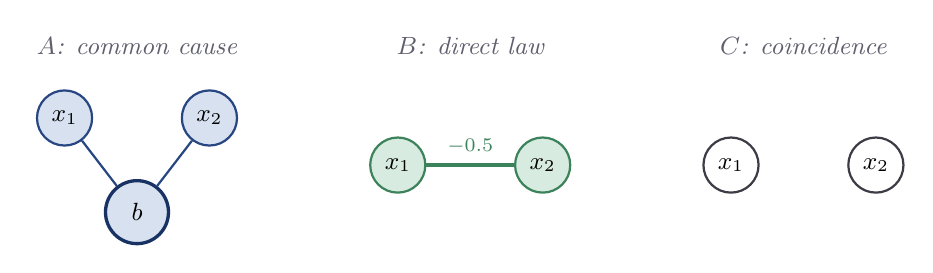
\begin{tikzpicture}[scale=0.92]
% A: common cause (star)
\begin{scope}
  \node[font=\small\itshape,notegrey] at (1,2.0) {$A$: common cause};
  \node[circle,draw=coreblue,thick,fill=softblue,minimum size=7mm,font=\small](a1) at (0,1){$x_1$};
  \node[circle,draw=coreblue,thick,fill=softblue,minimum size=7mm,font=\small](a2) at (2,1){$x_2$};
  \node[circle,draw=coredeep,very thick,fill=softblue,minimum size=8mm,font=\small](ab) at (1,-0.3){$b$};
  \draw[coreblue,thick](a1)--(ab); \draw[coreblue,thick](a2)--(ab);
\end{scope}
% B: direct law
\begin{scope}[xshift=4.6cm]
  \node[font=\small\itshape,notegrey] at (1,2.0) {$B$: direct law};
  \node[circle,draw=paradigmB,thick,fill=softB,minimum size=7mm,font=\small](b1) at (0,0.35){$x_1$};
  \node[circle,draw=paradigmB,thick,fill=softB,minimum size=7mm,font=\small](b2) at (2,0.35){$x_2$};
  \draw[paradigmB,very thick](b1)--(b2) node[midway,above,font=\scriptsize]{$-0.5$};
\end{scope}
% C: coincidence
\begin{scope}[xshift=9.2cm]
  \node[font=\small\itshape,notegrey] at (1,2.0) {$C$: coincidence};
  \node[circle,draw=darkgrey,thick,fill=white,minimum size=7mm,font=\small](c1) at (0,0.35){$x_1$};
  \node[circle,draw=darkgrey,thick,fill=white,minimum size=7mm,font=\small](c2) at (2,0.35){$x_2$};
\end{scope}
\end{tikzpicture}
\caption{Three candidate paradigms for one observed regularity between
$x_1$ and $x_2$: a hidden common cause ($A$), a direct law ($B$), or
coincidence ($C$). $B$ is exactly $A$ with the hidden cause marginalized
out --- its $-0.5$ edge is $A$'s carry-over.}
\label{fig:abc-nets}
\end{figure}

\paragraph{$A\to B$ is the carry-over (Schur complement).} Write $A$'s
precision in the ordering $(x_1,x_2,b)$, with unit couplings to the hub:
\begin{equation}
\Pi_A=\begin{pmatrix}2&0&1\\0&2&1\\1&1&2\end{pmatrix}.
\end{equation}
The hub is hidden, so to compare $A$ with the others on what is observed
we integrate it out. The effective precision over $(x_1,x_2)$ is the
Schur complement,
\begin{equation}
\Pi_A^{\mathrm{marg}}
=\begin{pmatrix}2&0\\0&2\end{pmatrix}
-\tfrac12\begin{pmatrix}1\\1\end{pmatrix}\begin{pmatrix}1&1\end{pmatrix}
=\begin{pmatrix}\,1.5&-0.5\,\\[1pt]\,-0.5&1.5\,\end{pmatrix}.
\end{equation}
A direct $-0.5$ coupling is \emph{born} between $x_1$ and $x_2$ where $A$
had none, and each self-precision falls $2\to1.5$. But that matrix is
exactly what paradigm $B$ posits as its direct law. So \textbf{$B$ is $A$
with the hidden cause marginalized away}: the carry-over edge of $A$ is
the law of $B$. The chain $A\to B$ is one Schur step.

\paragraph{Underdetermination: $A$ and $B$ are observationally
equivalent.} Because $B$ \emph{is} the marginal of $A$ over $(x_1,x_2)$,
the two assign identical evidence to any data about $x_1$ and $x_2$
alone. No amount of watching the two commitments can separate a common
cause from a direct law --- the reduced free energy
$\Delta F_{A\to B}=0$ on this marginal. To break the tie the hidden cause
must have \emph{its own} observable consequences: extra channels that $b$
predicts and a bare $x_1$--$x_2$ law does not. This is the role of a
heavily-connected core node --- the kind one stars as ``important'' and
wires to additional observations: those extra edges are precisely what
make $A$ falsifiable against $B$. Sample them and $A$'s evidence either
pulls ahead, if the common-cause structure is real, or it does not, in
which case parsimony keeps $B$.

\paragraph{$B\to C$ is BMR pruning.} Paradigm $C$ is $B$ with the $-0.5$
edge pruned --- its prior precision tightened to a spike at zero,
$\Pi_C=\mathrm{diag}(1.5,1.5)$. Now the reduced free energy of Step~5,
$\Delta F=\ln[\tilde p(o)/p(o)]-\Delta U$ (Eq.~\ref{eq:bmr}), is not zero:
the edge carries evidence whenever the correlation is real, so pruning it
costs evidence ($\Delta F<0$) and $B$ is kept; but if $x_1,x_2$ are in
fact uncorrelated, the posterior over the coupling has collapsed to zero
on its own, pruning refunds the edge's complexity cost ($\Delta F>0$),
and $C$ wins by Occam. (In the paper's categorical setting this
$\Delta F$ is the Dirichlet/Beta form of \citet{Friston2018_2}; the
Gaussian numbers here are for visibility.)

\paragraph{The dynamics: which paradigm leads, and when.} Put the three
running log-evidences on one axis (Figure~\ref{fig:abc-dyn}). Early, with
little data, $C$ leads: it spends no complexity on a coupling the data
have not yet demanded (Occam). As correlation data accumulate the $-0.5$
coupling earns its keep and $B$ overtakes $C$. $A$ tracks $B$ exactly ---
they are observationally equivalent --- until the hidden cause's extra
consequences are sampled, at which point $A$ overtakes $B$ if the common
cause is real. And if the world changes --- the hidden cause switches
off, leaving only a residual direct coupling --- $B$ retakes the lead
from $A$: a paradigm shift, read straight off the crossing of the
evidence curves.

\begin{figure}[ht]
\centering
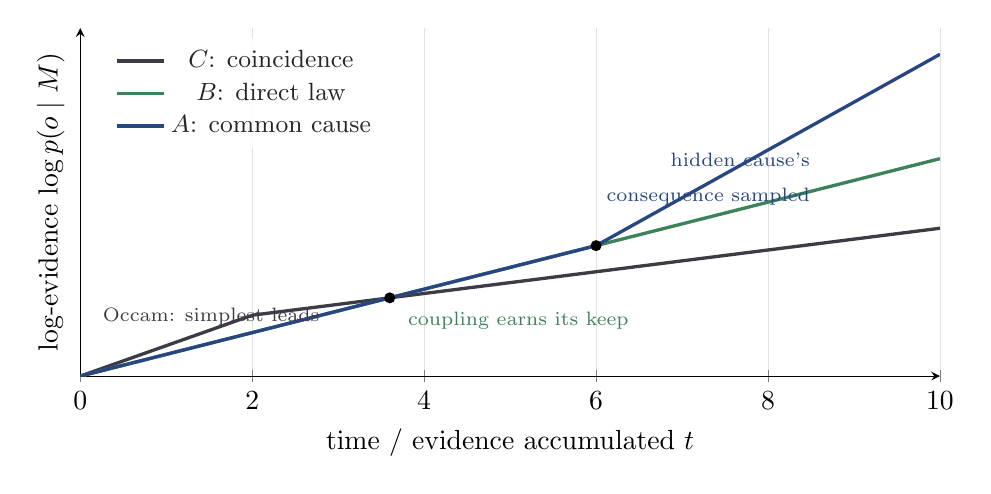
\begin{tikzpicture}
\begin{axis}[width=12.5cm,height=6cm,
  xlabel={time / evidence accumulated $t$},
  ylabel={log-evidence $\log p(o\mid M)$},
  xmin=0,xmax=10,ymin=0,ymax=8,xtick={0,2,4,6,8,10},ytick=\empty,
  axis lines=left,grid=major,grid style={notegrey!18,very thin},
  legend pos=north west,legend style={font=\small,draw=none,fill=white,fill opacity=0.85},
  every axis plot/.append style={very thick}]
% C: leads early (Occam), then flattens
\addplot[darkgrey,domain=0:10,samples=120]{0.7*x-0.45*max(0,x-2)};
\addlegendentry{$C$: coincidence}
% B: direct law
\addplot[paradigmB,domain=0:10,samples=120]{0.5*x};
\addlegendentry{$B$: direct law}
% A: tracks B until t=6, then pulls ahead
\addplot[coreblue,domain=0:10,samples=120]{0.5*x+0.6*max(0,x-6)};
\addlegendentry{$A$: common cause}
% crossings
\fill[black] (axis cs:3.6,1.8) circle (2pt);
\fill[black] (axis cs:6,3.0) circle (2pt);
\node[font=\scriptsize,darkgrey,anchor=south west] at (axis cs:0.15,0.95) {Occam: simplest leads};
\node[font=\scriptsize,paradigmB,anchor=north west] at (axis cs:3.7,1.7) {coupling earns its keep};
\node[font=\scriptsize,coreblue,anchor=south east] at (axis cs:8.6,4.6) {hidden cause's};
\node[font=\scriptsize,coreblue,anchor=north east] at (axis cs:8.6,4.55) {consequence sampled};
\end{axis}
\end{tikzpicture}
\caption{The three candidate paradigms as drifting log-evidences
(schematic). $C$ leads early by parsimony; $B$ overtakes once the
correlation is established; $A$ tracks $B$ until the hidden cause's extra
consequences are sampled, then overtakes if the common cause is real.
Each crossing (dots) is a model-selection paradigm shift.}
\label{fig:abc-dyn}
\end{figure}

\paragraph{Reading it back onto precision-corner navigation.} The chain
$A\to B\to C$ is a single trajectory through the precision space of
Figure~\ref{fig:bmr}: $A$ in the higher-dimensional interior (hub
present), $B$ at the face where the hub is marginalized (the carry-over
edge live), $C$ at the corner where that edge is pruned to zero. BMR is
the agent walking that trajectory, and the carry-over is why the walk is
not free: marginalizing the hub does not delete it, it deposits the
$-0.5$ law that $C$ must then pay evidence to remove. The three Kuhnian
readings of one regularity --- deep cause, brute law, coincidence ---
are three stations on that walk, and the data decide where the agent
stops.


\bibliographystyle{plainnat}
\bibliography{refs}

\end{document}
